\documentclass[preprint]{sigplanconf}

\usepackage{ifxetex}
\usepackage{amsmath}
\ifxetex
\else
  \usepackage[utf8]{inputenc}
\fi
\usepackage{listings}
\usepackage{tabularx}
\usepackage{url}
\usepackage{xspace} 
   
\usepackage{graphicx} 

\begin{document}

\newcommand*{\rb}{\textsc{Rootbeer}\xspace}
\newcommand*{\sootclass}{\texttt{SootClass}\xspace}
\newcommand*{\sootmethod}{\texttt{SootMethod}\xspace}
\newcommand*{\sootfield}{\texttt{SootField}\xspace}

% From http://en.wikibooks.org/wiki/LaTeX/Source_Code_Listings
\lstset{
  basicstyle=\footnotesize\tt,        % the size of the fonts that are used for the code
  breakatwhitespace=false,         % sets if automatic breaks should only happen at whitespace
  breaklines=true,                 % sets automatic line breaking
  captionpos=b,                    % sets the caption-position to bottom
  extendedchars=true,              % lets you use non-ASCII characters; for 8-bits encodings only, does not work with UTF-8
  frame=single,                    % adds a frame around the code
  language=Java,                 % the language of the code
  keywordstyle=\bf,
  showspaces=false,                % show spaces everywhere adding particular underscores; it overrides 'showstringspaces'
  showstringspaces=false,          % underline spaces within strings only
  showtabs=false,                  % show tabs within strings adding particular underscores
  tabsize=2                       % sets default tabsize to 2 spaces
}

\conferenceinfo{SOAP '13}{June 20th 2013, Seattle, Washington, USA } 
\copyrightyear{2013} 
\copyrightdata{[to be supplied]} 

\title{Soot Class Loading in the \rb GPU Compiler}
%\subtitle{Subtitle Text, if any}

\authorinfo{Philip C. Pratt-Szeliga}
           {Syracuse University\\Syracuse, NY, USA}
           {pcpratts@syr.edu}

\authorinfo{Marc-André Laverdière}
           {TCS Innovation Labs,\\Tata Consultancy Services, Ltd.\\\&\\
			École Polytechnique de Montréal\\
			Montréal, Canada}
           {marc-andre.laverdiere-papineau@polymtl.ca}

          
           
\authorinfo{Ettore Merlo}
           {École Polytechnique de Montréal\\
			Montréal, Canada}
           {ettore.merlo@polymtl.ca}           
           
\authorinfo{James W. Fawcett}
           {Syracuse University\\Syracuse, NY, USA}
           {jfawcett@twcny.rr.com}        
 
\authorinfo{Roy D. Welch}
           {Syracuse University\\Syracuse, NY, USA}
           {rowelch@syr.edu}       
    
           
%\authorinfo{Name2\and Name3}
%           {Affiliation2/3}
%           {Email2/3}

\maketitle

\begin{abstract}
One of the first activities of the Soot program analysis framework is to load 
the classes for analysis. With the current class loader, more classes are loaded
than necessary. These extra classes can consume too much memory during whole program
analysis making analysis infeasible on systems with four gigabytes of ram. This paper 
describes new algorithms and data structures to efficiently load Java
Bytecode classes for whole program analysis in Soot. Our method uses a modified 
version of Rapid Type Analysis (RTA) to determine what classes, methods and 
fields would be reachable during program execution. This enables us to load 
significantly less information in memory to enable program analyses.
We implemented our approach for loading Java bytecode in the Soot-based \rb 
compiler. The new class loader can load Scenes that are 64.94\% smaller and uses less than four gigabytes of ram for our test cases.
\end{abstract}

\category{D.3.4}{Programming Languages}{Processors – code generation}[compilers]

\terms
Algorithms, Performance, Design

\keywords
class loading; Soot; Java Bytecode

\section{Introduction}
\label{sec:intro}
Class loading in Soot \cite{soot-retro, soot-orig} can require significant time 
and memory when using whole-program mode. The current algorithm loads all 
classes from the process path and any class transitively referenced from loaded 
classes. All methods in a class are loaded whether or not they exist in any 
possible program traces. The number of loaded types starts out small, but as 
each class is loaded, more and more unnecessary types are added to the Scene. 
This results in a large memory footprint for analyzing even small programs, 
making some analyses impossible on lower-end systems.

To illustrate this issue, we introduce a running example in Listing \ref{lst:runningexample}.

%TODO add some fields and methods that are not needed so that we can show off even more.
\begin{lstlisting}[caption={Running example},label={lst:runningexample},float=!ht]
public class A {
  public static void main(String[] args){
    B b = new B();
    b.foo();
  }
}
public class B {
  public void foo(){
    C c = new C();
    c.abc();
  }
  public void bar(){
    D d = new D();
    d.abc();
  }
}
public class C {
  public void abc(){
    System.out.println("In class C");}
}
public class D {
  public void abc(){
    System.out.println("In class D");}
}
\end{lstlisting}

When loading this program in Soot in whole-program mode, without exclusions, the class loader fully loads 2031 \sootclass objects. With the \rb class loader it loads 712 \sootclass objects, representing an approximate reduction of 114 Mb in memory usage.

%Do we add more, like Body or Unit?

We include an illustration of a subset of the dependencies loaded with the current class loader for our running example in Figure \ref{fig:deps}. While significantly truncated, and slightly unreadable, it shows that even trivial programs require a significant number of core Java classes to be loaded in memory.

\begin{figure}

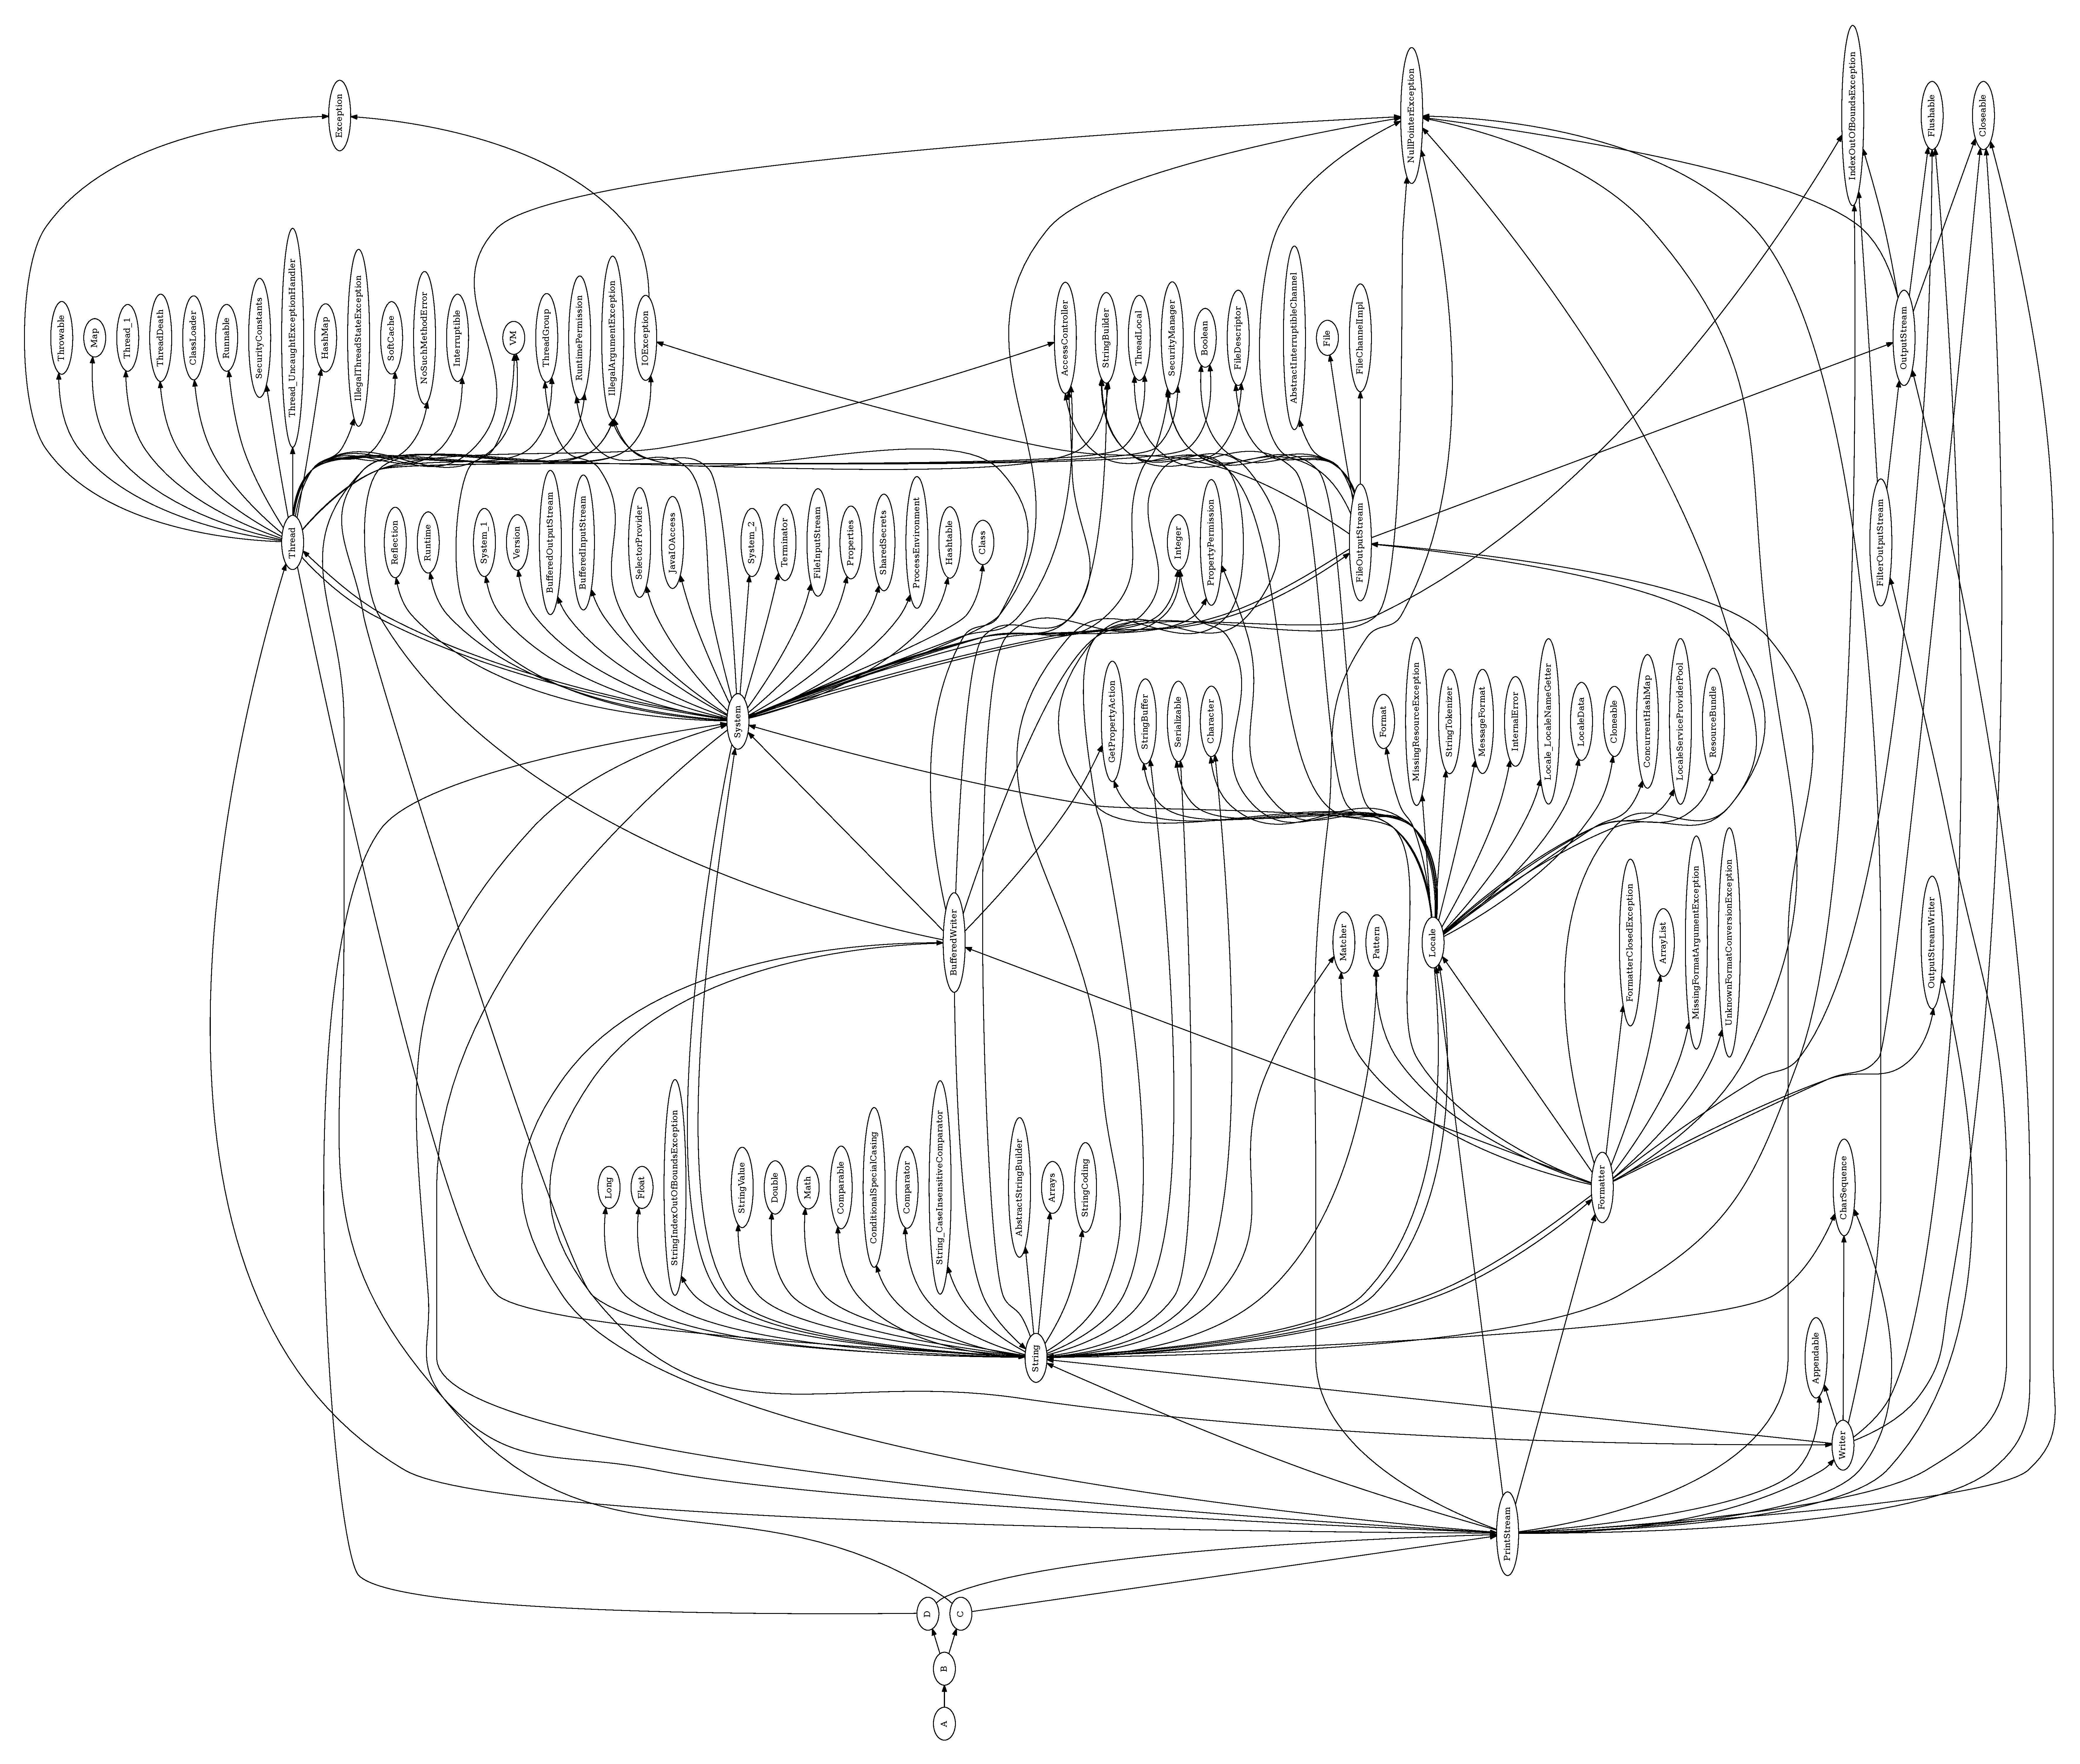
\includegraphics[scale=0.08,angle=-90]{class-dependency-small.pdf} 

\caption{Subset of Class Dependencies for Listing \ref{lst:runningexample}}
\label{fig:deps}
\end{figure}
This paper describes a new class loading algorithm and the required data structures to only load the set of classes that would be needed during program execution. Our strategy is to gather information from the Coffi bytecode representation without creating the Soot internal objects, while we build an over-approximate call graph. Once all of the reachable classes have been discovered, the types are numbered according to the class hierarchy and we load a minimal Scene.

We have implemented this scheme in the \rb GPU Compiler \cite{rootbeer}. 

The contents are organized as follows. In section \ref{sec:new-cl}, we will first describe the current Soot class loading algorithm and why it has problems with memory usage. Then, in section \ref{sec:new-cl}, we will describe our methodology and describe the new class loading algorithm in detail. Then, in section \ref{sec:api}, we describe the new API added to Soot. We then compare the performance of our method with Soot's class loading in \rb in section \ref{sec:eval}. Finally, in section \ref{sec:future}, we will discuss future work, and conclude in section \ref{sec:conclusion}.

%TODO merge some of  that in the introduction ?
\section{Soot Whole-Program Class Loading}
\label{sec:soot-cl}

The original Soot class loading algorithm has three basic resolving levels: Hierarchy, Signatures and Bodies. As the level of a class progresses from Hierarchy to Bodies, additional details are loaded from the class files to memory. Table \ref{tbl:resolving_levels} summarizes the information added at each resolving level. 

\begin{table}
\begin{tabularx}{\columnwidth}{|l|X|}
\hline
\textbf{Resolving Level} & \textbf{Associated Information} \\\hline
Dandling  & Nothing is known about the class, except its fully-qualified name.\\\hline
Hierarchy & The class, its superclass and interfaces are loaded. \\\hline
Signatures & Hierarchy information, as well as types declared in method signatures and fields. \\\hline
Bodies & Signatures information, as well as the classes referenced in the method bodies. \\\hline
\end{tabularx}
\caption{Resolving levels in Soot}
\label{tbl:resolving_levels}
\end{table}

We now describe the class loading algorithm with more details, without including information related to phantom reference support\footnote{Phantom references are classes that are not resolved, either because they are not found in the class path, or have been excluded.}.
The Soot resolver will work incrementally in the Scene, by means of a worklist\footnote{There are four worklists, but their behavior is identical in whole-program mode, so we merge them as one for simplicity}, by loading each class and its dependencies, one at a time.

Note that the steps below are repeated for every class in the process path and every basic class. Please note also that every step has an early termination feature if the class is determined to be at the given level already.

The algorithm is initialized in the {\tt resolveClass} method with an empty \sootclass container object at the Dandling level. This empty container is then added to the desired resolving level.

In the first phase, Soot loads the class to the hierarchy level. First, the class source (Coffi, Jimple, etc.) is loaded into the \sootclass object.
The \sootclass objects of the outer class, the super class and the interfaces are added to the worklist. The corresponding {\tt Type} instances are created and stored for later use.

In the second phase, Soot loads the class to the signature level. It does so by examining the hierarchy anew, the methods signatures and the fields. All classes identified in the fields and signatures (including the return type, the arguments and the declared exceptions) are added to the worklist.

In the third phase, Soot resolves the class at the bodies level. Note that all initialization statements in Java code are automatically moved to the appropriate initializer, so that every executable statement is in a method body. Soot uses the information stored as {\tt Type} in the first step and adds it all to the worklist.

The weakness of this algorithm is its all-or-nothing nature. It loads all the classes that are reachable from the basic classes and the processable classes, irrespective of whether they would be used in the program or not.

For our running example (c.f. Listing \ref{lst:runningexample}), this algorithm loads the classes A,B,C and D, as well as a large amount of JDK classes.

\section{Class Loading using RTA}
\label{sec:new-cl}
Our class loading strategy is to keep class names, method bodies as well as method and field signatures as strings for as long as possible.
The \sootclass, \sootmethod, \sootfield and {\tt Body} objects are only created once the types are numbered. Another important part of our strategy is that we load classes that are found on a depth first search walk from the entry points.

For our running example (c.f. Listing \ref{lst:runningexample}), this algorithm loads the classes A,B and C, as well as a restricted set of JDK classes. %TODO details here

We explain the initial class loading step in section \ref{sec:loading}, followed by the construction of the call graph in section \ref{sec:cg}. Then, we explain some special features of \rb and how we accommodate them in our class loading scheme in section \ref{sec:followtosig}. Afterwards, we explain the class numbering algorithm in section \ref{sec:numbering} and how the {\tt Scene} object is populated in section \ref{sec:loadscene}.

\subsection{Load and Wrap Classes}
\label{sec:loading}
The first step of our algorithm uses the list of classes in the process path and loads them in memory using Coffi. We convert the constant pool indices for the current class, super class and interfaces into a string representation. We put all this information into a wrapper class named {\tt HierarchySootClass} and store them in a map (with the class name as key) for fast lookups.

\subsection{Building a Call Graph}
\label{sec:cg}
In order to know which classes are reacheable in a normal program execution, we build a call graph of the program using a bi-directional variation of the optimistic Rapid Type Analysis (RTA) algorithm \cite{BaconRTA, Sundaresan:2000:PVM:354222.353189}.

We chose RTA as our base because it is a very fast algorithm that doesn't require us to perform any flow analyses, making it suited for the low-information phase we are in.

The original optimistic RTA algorithm uses Class Hierarchy Analysis (CHA) \cite{deanetal} to bootstrap a traversal of the program from the entry point. While the program is traversed, the class instantiations detected are recorded, and only the call targets that correspond to the found classes are preserved. This algorithm executes as a fixed point over the number of new class invocations.

However, this algorithm needs to be modified to fit our needs. First, RTA presumes a single entry point at the root of the program execution. In our case, however, we allow multiple entry points, which may not be at the start of the program execution. %We need to justify why that is important.

Our variation of RTA is also bootstrapped by CHA. As such, we will not go in the details of the construction of the class hierarchy and the virtual method resolution cache.

Note that this traversal can be bounded, resulting in a truncated call graph. While is unsound, it is often useful in practice. The mechanism for evaluating whether to visit a node is called the \emph{don't follow} set.

\subsubsection{Entry Points}
The first step in building a call graph is to determine the entry points. Our class loader provides a flexible entry point mechanism. Soot users who analyze software that does not have a {\tt main} method need not generate one for the sake of analysis, but simply need to create an appropriate {\tt MethodTester} class and register it with the {\tt RootbeerClassLoader.addEntryMethodTester} method. All the details of this API is provided in section \ref{sec:api}.

Our class loader submits all the methods found in the previous steps to the registered method testers. If any of the testers return true, then this method is considered as an entry point.

\subsubsection{Forward Traversal}

During the forward traversal, we start at the entry points and traverse program using a breadth-first search. Along the way, we record all constructor invocations. Since we do not load instructions to Jimple, we use the {\tt HierarchyValueSwitch} API described in section \ref{sec:api}.
When a constructor call to a new class is found, its virtual methods are placed on the call graph and the virtual method cache.

To make the backward traversal rapid, the forward traversal maintains the \emph{reachable set}, which is the set of all reacheable methods. This set is seeded with the entry points and we add the signature of every method that is found reacheable.

%How do we handle non-static entry points.

\subsubsection{Backward Traversal}
If an entry point is not a main function, all of the methods on a depth first search walk from a main to the entry point need to be loaded in order to accurately represent the runtime behaviour.

This is handled by a backward traversal from the entry points. When traversing the methods, we examine, using the \emph{reachable set}, if it contains any method call to any methods in the call graph. If so, the edge is added to the call graph.

\subsubsection{Convergence}
Since our algorithm is monotonic (only new virtual call targets are added) and the number of classes loaded is finite, we are guaranteed to converge. Note that we use the number of constructor invocations found for determining the fixed point, as this is more economical to use than graph comparison and simpler to implement than many of the options suggested by Lhoták \cite{lhot02}.

\subsection{\rb{}-Specific Overrides}
\label{sec:followtosig}

The \rb GPU Compiler needs additional information in the loaded {\tt Scene} that would not be present in the classes loaded previously.

Firstly, \rb needs a mechanism to handle entry points determined by reflection, which \rb uses. These are called \emph{follow methods} and \emph{follow classes}. Note that \emph{follow methods} could also be used to model other non-explicit entry points, such as {\tt Thread.run} entry points. These are added to the set of entry points when the call graph is constructed.

Secondly, \rb also needs its runtime classes to be loaded to signatures (i.e. with no method bodies) so that the generated Jimple code can refer to the runtime methods. The set of \emph{to-signature classes} and \emph{methods} allows this.

All the overrides mentioned are configured with {\tt MethodTester}s and {\tt ClassTester}s. The \emph{follow testers} and \emph{to-signature testers} are evaluated once to save time.

\subsection{Numbering Types}
\label{sec:numbering}
The Soot framework requires a unique number on many kinds of objects, including \sootclass instances.

After the call graph is created, the types are numbered as follows. The number starts at one for the root Java {\tt Object}. Afterwards, we number the interfaces in reverse topological order. Then, we number the remaining classes using a breadth-first traversal on the hierarchy.

We use topological sorting for the interfaces because of the fact that all interfaces inherit from {\tt Object} in the strict sense, even though they may extend many other interfaces. A breadth-first numbering approach would yield broken dependencies in the next step, which this approach solves. 

\subsection{Load Scene}
\label{sec:loadscene}
The final stage of the algorithm is to load the Scene. 

The loading happens in four steps: loading the hierarchy, loading reachable fields, loading reachable methods, and finally the method bodies are loaded from Coffi.

These steps are necessary because the \sootclass, \sootfield and \sootmethod instances reachable from the bodies must exist before the body can be resolved.

As the last two steps are self-explanatory, we only explain the loading of the hierarchy and of the reachable fields.

In the first step, the numbered types are visited from smallest to largest and empty \sootclass objects are created. At each empty \sootclass object the super class and interfaces are filled in. The super class and interfaces are retrieved from the {\tt Scene} by calling {\tt Scene.getSootClass}. Since the numbering is according to the class hierarchy, the object classes are guaranteed to already exist in the {\tt Scene}.

In the second step, we traverse the program to find all the field references. We parse the string-based information with \\*
{\tt FieldSignatureUtil} and construct the appropriate \sootfield object. This field object is then added to the declaring \sootclass.
%TODO do we really parse the whole program for this.

%TODO are we loading only the methods that are reacheable???

Note that this approach results in a subset of the classes loaded, and a subset of the class details being converted to Jimple. Since our call graph is sound, no information is missing that would be required during program execution.

In the case of our running example, we would have a lighter scene loaded, as illustrated in Listing \ref{lst:loadscenerunningexample}. Please note that JDK library classes were not added in. We notice that the class {\tt B} does not have the {\tt bar()} method, nor is the class {\tt D} loaded.

\begin{lstlisting}[caption={Loaded Scene for Running example},label={lst:loadscenerunningexample},float=!ht]
public class A {
  public static void main(String[] args){
    B b = new B();
    b.foo();
  }
}
public class B {
  public void foo(){
    C c = new C();
    c.abc();
  }
}
public class C {
  public void abc(){
    System.out.println("In class C");}
}
\end{lstlisting}

\section{New API}
\label{sec:api}
To create the \rb class loader, a new API was needed that supported string data structures. This section gives a summary of each method included with the \rb class loader.

Note that analyses in Soot will not need to refer to these APIs, as the class loader eventually brings the Coffi data to the familiar classes.

The {\tt RootbeerClassLoader} is a singleton with the entry point to class loading ({\tt loadNecessaryClasses}). You can configure the entry points by adding a {\tt MethodTester}. Please refer to Figure \ref{fig:rbcl} for the details of the methods offered.

\begin{figure*}[htbf]

\begin{tabularx}{\textwidth}{|XX|}
\hline
{\bf Method} & {\bf Description }\\\hline
{\tt void loadNecessaryClasses()} &  Load the Scene \\\hline
{\tt ClassHierarchy getClassHierarchy()} & Get the class hierarchy data structure\\\hline
{\tt List<SootMethod> getEntryPoints()} & Get the \sootmethod entry points that were specified using the MethodTesters\\\hline
{\tt void addEntryMethodTester (MethodTester mt)} & Add a MethodTester that will be used to define entry points\\\hline
{\tt void addFollowMethodTester (MethodTester mt)} & Add a MethodTester that will be used to include methods in the reachable walk\\\hline
{\tt void addFollowClassTester (ClassTester ct)} & Add a ClassTester that will be used to include classes in the reachable walk\\\hline
{\tt void addDontFollowMethodTester (MethodTeter mt)} & Add a MethodTester that will stop a reachable walk\\\hline
{\tt void addDontFollowClassTester (ClassTester ct)} & Add a ClassTester that will stop a reachable walk\\\hline
{\tt void addToSignaturesMethodTester (MethodTester mt)} & Add a MethodTester that will define methods to be raised to signatures\\\hline
{\tt void addToSignaturesClassTester (ClassTester ct)} & Add a ClassTester that will define classes to be raised to signatures\\\hline
\end{tabularx}
\caption{{\tt RootbeerClassLoader} API}
\label{fig:rbcl}
\end{figure*}


The {\tt ClassHierarchy} (see Figure \ref{fig:rbch}) is reachable from the {\tt RootbeerClassLoader} singleton. It allows a developer to retrieve the virtual methods for a signature, get a {\tt HierarchyGraph} for a class name, get a {\tt HierarchyClass} and get the {\tt NumberedTypes}.

\begin{figure*}[htbf]
\begin{tabularx}{\textwidth}{|XX|}
\hline
{\bf Method} & {\bf Description }\\\hline
{\tt boolean containsClass(String name)} & Returns true if the 
    class name is loaded \\\hline
{\tt List<String> getAllVirtualMethods(String signature)} & 
    Return the virtual method signatures with the same 
    covariant subsignature for all classes where new has been 
    invoked on the string call graph\\\hline
{\tt HierarchyGraph getHierarchyGraph(String className)} & 
    Gets a HierarchyGraph for a class name\\\hline
{\tt HierarchyClass getHierarchyClass(String className)} & 
    Gets a HierarchyClass for a class name\\\hline 
{\tt List<NumberedType> getNumberedTypes()} & Get the 
    numbered types in ascending order\\\hline
{\tt Set<String> getAllClasses()} & Get all of the classes in the
    class hierarchy\\\hline
\end{tabularx}
\caption{{\tt ClassHierarchy} API}
\label{fig:rbch}
\end{figure*}


The {\tt MethodTester} interface is designed to be implemented by classes that can tell if a {\tt HierarchyMethod} meets a criteria. It has a single method, {\tt boolean test(HierarchyMethod sm)}, which returns true if the criterion is met.

The {\tt ClassTester} interface is similar to {\tt MethodTester}, except that it can be used to see if a {\tt HierarchyClass} meets a class or package criterion. It has a single method, {\tt boolean test(Hierarchy\-Class sm)}. The {\tt RootbeerClassLoader} calls the {\tt ClassTester} once per class and the {\tt MethodTester} once per method.
%Not true, because of the don't follow strings

The {\tt HierarchyClass} keeps the class name, super class name and interfaces as strings. It can return all of the {\tt HierarchyMethods} or find them by name or sub-signature. Its methods are described in Figure \ref{fig:rbhc}.

\begin{figure*}[htbf]
\begin{tabularx}{\textwidth}{|XX|}
\hline
{\bf Method} & {\bf Description }\\\hline
{\tt HierarchyMethod getMethodByName(String name)} &  Searches for a 
    method by name\\\hline
{\tt HierarchyMethod getMethodBySubSignature(String subSig)} & 
    Searches for a method by subsignature\\\hline
{\tt List<String> getInterfaces()} & Get the interfaces as a string \\\hline
{\tt List<HierarchyMethod> getMethods()} & Get the methods\\\hline
{\tt HierarchyMethod getMethodCovarient(String css)} & Get the
    HierarchyMethod matching the input covariant subsignature\\\hline
{\tt String getName()} & Get the name of the class\\\hline
{\tt String getSuperClass()} & Get the name of the super class\\\hline 
{\tt boolean hasSuperClass()} & Returns true if the class has a 
    super class\\\hline
\end{tabularx}
\caption{{\tt HierarchyClass} API}
\label{fig:rbhc}
\end{figure*}

The {\tt HierarchyMethod} keeps the method name, return type, parameter types and exception types as strings. It can return the bytecode instructions of a method as {\tt HierarchyInstructions}. The {\tt HierarchyInstructions} are string based representations of the bytecode. The method signature and sub-signature can be obtained. The class is described in Figure \ref{fig:rbhm}.

\begin{figure}[htbf]
\begin{tabularx}{\columnwidth}{|XX|}
\hline
{\bf Method} & {\bf Description }\\\hline
{\tt List<String> getExceptionTypes()} &  Returns the exceptions\\\hline 
{\tt HierarchyClass getHierarchyClass()} & Get
   the declaring HierarchyClass\\\hline 
{\tt List
    <HierarchyInstruction>
    getInstructions()} & Get the 
    Instructions of the method in a string based format\\\hline 
{\tt String getName()} & Get the name of the method\\\hline 
{\tt List<String> getParameterTypes()} & Get the types of the parameters\\\hline
{\tt String getReturnType()} & Get the return type\\\hline
{\tt String getSignature()} & Get the signature of the method\\\hline  
{\tt String getSubSignature()} & Get the subsignature of the method\\\hline
{\tt String getCovarientSignature()} & Get the covariant subsignature of the method\\\hline
\end{tabularx}
\caption{{\tt HierarchyMethod} API}
\label{fig:rbhm}
\end{figure}

The {\tt HierarchyInstruction} has two methods. The first is {\tt String getName()}, which keeps track of the name of the instruction (like “new”). The second is {\tt List<Operand> getOperands()}, representing the string-based {\tt Operand}.

The {\tt Operand} class keeps track of the instruction operand as converted to a string using the class constant pool. It keeps track of a string-based type that allows easy searching for class\_refs, method\_refs and field\_refs. Its description is available in Figure \ref{fig:operand}. 

\begin{figure}[htbf]
\begin{tabularx}{\columnwidth}{|lX|}
\hline
{\bf Method} & {\bf Description }\\\hline
{\tt String getValue()} &  Returns, as a string, the operand parsed 
    from the constant pool\\\hline 
{\tt String getType()} & Returns a type of the value. Can be one
    of the following:
    \begin{description}
      \item[basic types] byte, int, long, float, double, string
      \item[descriptor types] class\_ref, method\_ref, field\_ref
    \end{description}
\\\hline 
\end{tabularx}
\caption{{\tt Operand} API}
\label{fig:operand}
\end{figure}

The {\tt HierarchyValueSwitch} takes a method signature and processes each {\tt HierarchyInstruction}. It records types, method and field references and new invokes. It is described in Figure \ref{fig:hvsw}

%TODO give the details of what those strings are going to be like?
\begin{figure}[htbf]
\begin{tabularx}{\columnwidth}{|lX|}
\hline
{\bf Method} & {\bf Description }\\\hline
{\tt Set<String> getRefTypes()} &  Get reference types\\\hline
{\tt Set<String> getTypes()} &  Get all types\\\hline
{\tt Set<String> getArrayTypes()} &  Get array types\\\hline
{\tt Set<String> getMethodRefs()} &  Get method refs\\\hline
{\tt Set<String> getFieldRefs()} &  Get field refs\\\hline
{\tt Set<String> getNewInvokes()} &  Get new invokes\\\hline
\end{tabularx}
\caption{{\tt HierarchyValueSwitch} API}
\label{fig:hvsw}
\end{figure}

There is one {\tt HierarchyGraph} instance per class name. It allows the developer to retrieve all classes in the hierarchy, the direct children of a parent class and the parents of a child class. It is described in Figure \ref{fig:hg}.

\begin{figure}[htbf]
\begin{tabularx}{\columnwidth}{|XX|}
\hline
{\bf Method} & {\bf Description }\\\hline
{\tt List<String> getAllClasses()} &  Get all the classes in the 
    hierarchy graph\\\hline
{\tt List<String> getChildren (String parent)} &  Get the direct 
    children of a parent class or interface\\\hline
{\tt List<String> getParents (String child)} &  Get the direct
    parents of a child class or interface\\\hline
\end{tabularx}
\caption{{\tt HierarchyGraph} API}
\label{fig:hg}
\end{figure}

The {\tt StringCallGraph} (see Figure \ref{fig:scg}) keeps a mapping of edges going out of a method signature and methods hitting a method signature. It also can return all signatures and tell if a signature is on the call graph.

\begin{figure}[htbf]
\begin{tabularx}{\columnwidth}{|XX|}
\hline
{\tt Set<String> getAllSignatures()} & Get all reachable method 
    signatures in the call graph\\\hline 
{\tt Set<String> getForwardEdges(String sourceSig)} & Get the
    method signatures that the sourceSig method calls directly\\\hline  
{\tt Set<String> getReverseEdges(String destSig)} & Get the
    method signatures that call the destSig directly\\\hline
{\tt boolean isReachable(String signature)} & Returns true if the
    method signature is in the call graph\\\hline
\end{tabularx}
\caption{{\tt StringCallGraph} API}
\label{fig:scg}
\end{figure}

There are two remaining useful classes in the {\tt soot.\-rbclassload} package. {\tt MethodSignatureUtil} can parse a method signature and return its name and types as strings. Any part of a method signature can be modified and a \sootmethod can be returned. {\tt FieldSignatureUtil} can parse a field signature and return its parts. Also any part of a field signature can be modified and a \sootfield can be returned.

\section{Evaluation}
\label{sec:eval}
%TODO which options are we setting? Any dontfollow strings?

We have implemented our algorithm inside the \rb{}-specific fork of Soot. We currently only load from Java bytecode. The code is available online\footnote{\url{https://github.com/pcpratts/soot-rb}} and we hope to integrate it in Soot in the near future.

%TODO put in the specs
We have executed the test cases on a 4 core Intel Xeon Processor (E5405) running at 2.00GHz with 16 Gb of RAM, running Linux 2.6.32-5-amd64 and JDK 1.6.0\_45 64-bit. 

Our test cases include our running example, and parts of the \rb test suite. We measured the execution time with Soot's built-in feature, and used the Classmexer\footnote{\url{http://www.javamex.com/classmexer/}} agent to measure the memory used by the loaded \sootclass objects. The overall memory usage was calculated using the JVM's global memory usage feature. The \rb tests (Soot) are marked NA because the original soot class loader crashed with a segmentation fault while loading.

%On my system, with soot loader
% Dandling: 0 Hierarchy: 0 Signatures: 0 Bodies: 2226. Num SootMethod: 21280
% Memory used in wjpp phase: 97.92635 Mb	Memory used for SootClass objects: 29.016594 Mb Scene size: 29.614433 Mb
% Memory used in wjtp phase: 299.9101 Mb	Memory used for SootClass objects: 96.312614 Mb Scene size: 130.69418 Mb
%       Resolving classfiles: 00.0s (00.0%)
% Bytecode -> jimple (naive): 06.5s (08.7%)

\begin{table}[htbf]
\begin{tabularx}{\columnwidth}{|p{1.5cm}|p{1cm}|X|X|l|}
\hline
\textbf{Test Case} & \textbf{Classes Loaded} & \textbf{Memory Used (Mb)} & \textbf{\sootclass Memory (Mb)}& \textbf{Time (s)} \\\hline
Running example (Soot) & 2031 & 885 & 139 & 91 \\\hline
Running example (RBC)  & 712  & 1357 & 25 & 105 \\\hline
\rb tests (Soot) & NA & NA & NA & NA \\\hline
\rb tests (RBC) & 1308 & 2586 & 35 & 225 \\\hline
\end{tabularx}
\caption{Experimental results}
\label{tbl:results}
\end{table}

We compare our implementation against the Soot class loader by loading programs and taking measurements in the wjpp phase in Table \ref{tbl:results}.

While we could have measured the overall memory used by the Java virtual machine at any given point, we chose not to because of the garbage collection's impredictability as well as the fact that newer garbage collectors typically work continuously in a separate thread. These factors make it essentially impossible to know what is the amount of memory really used in the program at a given point. This is the reason why we measured the \sootclass usage separately.

We notice a significant decrease in the number of classes loaded, which a minimal increase in processing time. It appears that the overhead of traversing the program in memory is only slightly greater than that of loading many files in memory. While we were careful about performance in our implementation, it is possible that further optimizations would allow us to break even in terms of loading time.

\section{Future Work}
\label{sec:future}
There are two aspects of future work that the \rb GPU Compiler is interested in working on. First, parallel cpu threads will be used to try and accelerate class loading. Second, a project named Jimple Web Cache may be created.

The Jimple Web Cache project aims to host a server online that can serve string based Jimple Bodies and StringCallGraphs. It will take an rt.jar (Java Runtime Jar) from the client and if it does not have a jar with the same name and md5 sum, it will cache the entire call graph of the archive in a MongoDB database along with the string based Jimple bodies. A user will be able to query to retrieve a call graph or Jimple body from an entry point method signature.

\section{Conclusion}
\label{sec:conclusion}
We have shown data structures and algorithms to efficiently load a Soot Scene in under 4 gigabytes of memory and 5 minutes time when doing whole-program analysis from an entry point. The Scene is about 26\% smaller and the memory savings are of about 82\%.

\acks
Philip C. Pratt-Szeliga was supported by Syracuse University and National Science Foundation grant number MCB-0746066 to R.D.W.

% We recommend abbrvnat bibliography style.

\bibliographystyle{abbrvnat}
\bibliography{bib}

% The bibliography should be embedded for final submission.
%TODO copy-paste the bib output in there
%\begin{thebibliography}{}
%\softraggedright

%\bibitem[1]{soot-retro} Patrick Lam and Eric Bodden and Ondrej Lhotak and Laurie Hendren. The Soot framework for Java program analysis: a retrospective. In: Cetus Users and Compiler Infastructure Workshop (CETUS 2011).
%\bibitem[2]{rootbeer} Philip C. Pratt-Szeliga, James W. Fawcett, Roy D. Welch. \rb: Seamlessly using GPUs from Java. HPCC-2012.
%\bibitem[3]{soot-orig} Raja Vallee-Rai and Phong Co and Etienne Gagnon and Laurie Hendren and Patrick Lam and Vijay Sundaresan. Soot - a Java bytecode optimization framework. Proceedings of the 1999 conference of the Centre for Advanced Studies on Collaborative research. 1999. IBM Press.
%\bibitem[4]{deanetal} Jeffrey Dean and David Grove and Craig Chambers. Optimization of Object-Oriented Programs
%Using Static Class Hierarchy Analysis, UW CSE Technical Report 94-12-01, 1994


%% TODO get the citatadd page numbers on those citations

%\end{thebibliography}

\end{document}
